\documentclass[12pt,a4paper]{article}

% Margin: atas 3cm, bawah 3cm, kanan 3cm, kiri 4cm, kertas A4
\usepackage[top=3cm,bottom=3cm,right=3cm,left=4cm,a4paper]{geometry}

\usepackage{graphicx}
\usepackage{listings}
\usepackage{xcolor}
\usepackage[hidelinks]{hyperref}
\usepackage{fancyhdr}
\usepackage{setspace}
\usepackage{indentfirst}
\usepackage{amsmath}
\usepackage{float}
\usepackage{multirow}
\usepackage{ragged2e}
\usepackage{titlesec}
\usepackage{caption}
\usepackage[indonesian]{babel}
\usepackage[none]{hyphenat}
\usepackage{microtype}

\sloppy
\emergencystretch=2em

% Semua teks utama 12pt, spasi 1.15, rata kiri-kanan
\setstretch{1.15}
\AtBeginDocument{\justifying\normalsize}

% Paragraf
\setlength{\parindent}{1.25cm}
\setlength{\parskip}{0pt}

% Section dan subsection tetap 12pt, hanya bold
\titleformat{\section}
  {\normalfont\normalsize\bfseries}
  {\thesection}{1em}{}

\titleformat{\subsection}
  {\normalfont\normalsize\bfseries}
  {\thesubsection}{1em}{}

\titleformat{\subsubsection}
  {\normalfont\normalsize\bfseries}
  {\thesubsubsection}{1em}{}

% Caption gambar/tabel juga 12pt
\captionsetup{
    font=normalsize,
    labelfont=bf
}

% Nama daftar isi
\renewcommand{\contentsname}{Daftar Isi}

% rename figure to Gambar
\renewcommand{\figurename}{Gambar}

% Style untuk listing kode
\definecolor{codegreen}{rgb}{0,0.6,0}
\definecolor{codegray}{rgb}{0.5,0.5,0.5}
\definecolor{codepurple}{rgb}{0.58,0,0.82}
\definecolor{backcolour}{rgb}{0.95,0.95,0.92}

\lstdefinestyle{mystyle}{
    backgroundcolor=\color{backcolour},
    commentstyle=\color{codegreen},
    keywordstyle=\color{magenta},
    numberstyle=\tiny\color{codegray},
    stringstyle=\color{codepurple},
    basicstyle=\ttfamily\footnotesize,
    numbers=left,
    numbersep=5pt,
    breaklines=true,
    breakatwhitespace=false,
    columns=fullflexible,
    keepspaces=true,
    showspaces=false,
    showstringspaces=false,
    showtabs=false,
    tabsize=2,
    captionpos=b,
    postbreak=\mbox{\textcolor{codegray}{$\hookrightarrow$}\space}
}
\lstset{style=mystyle}

\begin{document}

% Halaman Cover
\begin{titlepage}
    \thispagestyle{empty}
    \centering
    \vspace*{-1.2cm}

    {\normalsize\bfseries Laporan Mini Project\par}
    \vspace{0.25cm}
    {\normalsize\bfseries Lampu Berjalan, Kontrol LDR, Dimming, dan WiFi Scanner\par}

    \vspace{1.4cm}

    
\includegraphics[width=0.5\textwidth]{assets/img/logo-depart.png}

    \vspace{1.4cm}

    {\normalsize\bfseries Mata Kuliah\par}
    \vspace{0.2cm}
    {\normalsize Sistem Mikroprosesor dan Mikrokontroller\par}

    \vspace{0.8cm}

    {\normalsize\bfseries Dosen Pengampu\par}
    \vspace{0.2cm}
    {\normalsize Eko Pramunanto, S.T., M.T.\par}

    \vspace{1.1cm}

    {\normalsize\bfseries Disusun oleh\par}
    \vspace{0.25cm}
    {\normalsize Yuke Brilliant Hestiavin\par}
    {\normalsize 5024241016\par}

    \vfill

    {\normalsize
    Departemen Teknik Komputer\\
    Fakultas Teknologi Elektro dan Informatika Cerdas\\
    Institut Teknologi Sepuluh Nopember\\
    Surabaya, 3 Juni 2026
    \par}
\end{titlepage}

\pagenumbering{roman}
\tableofcontents
\newpage

\pagenumbering{arabic}

\section{Pendahuluan}

\subsection{Latar Belakang}
Sistem pencahayaan otomatis dan kontrol nirkabel merupakan salah satu contoh penerapan sistem embedded dalam kehidupan sehari-hari. Pada sistem tersebut, mikrokontroler digunakan untuk membaca input dari sensor, memproses data, dan menghasilkan output berupa kendali aktuator.

Mini project ini menggabungkan beberapa konsep utama dalam mata kuliah Sistem Mikroprosesor dan Mikrokontroller, yaitu Pulse Width Modulation (PWM), Analog to Digital Converter (ADC), sensor cahaya LDR, pembacaan potensiometer, dan konektivitas WiFi pada ESP32. Sistem yang dibuat berupa lampu berjalan atau efek Knight Rider dengan pengaturan kecepatan dan kecerahan, kontrol otomatis berbasis LDR, serta fitur pemindaian jaringan WiFi secara asinkron.

\subsection{Tujuan}
Tujuan dari mini project ini adalah sebagai berikut:
\begin{itemize}
    \item Menerapkan teknik PWM untuk mengontrol kecerahan LED.
    \item Menggunakan potensiometer sebagai input analog untuk mengatur brightness dan kecepatan animasi lampu.
    \item Mengimplementasikan sensor LDR sebagai kontrol otomatis berdasarkan intensitas cahaya lingkungan.
    \item Memahami penggunaan beberapa kanal ADC pada ESP32 untuk membaca beberapa input analog secara bersamaan.
    \item Mengimplementasikan fitur WiFi scanning secara asinkron atau non-blocking pada ESP32.
    \item Menampilkan hasil pembacaan sensor, potensiometer, dan WiFi scanner melalui Serial Monitor.
\end{itemize}

\section{Dasar Teori}

\subsection{Pulse Width Modulation (PWM)}
Pulse Width Modulation atau PWM adalah teknik untuk mengatur daya rata-rata yang diberikan kepada beban dengan cara mengubah perbandingan waktu aktif dan tidak aktif dari sinyal digital. Perbandingan waktu aktif terhadap satu periode sinyal disebut duty cycle.

Pada LED, duty cycle yang lebih besar akan menghasilkan nyala yang lebih terang, sedangkan duty cycle yang lebih kecil akan menghasilkan nyala yang lebih redup. Dengan teknik PWM, ESP32 dapat mengontrol kecerahan LED tanpa harus menggunakan rangkaian analog tambahan.

\subsection{Analog to Digital Converter (ADC)}
Analog to Digital Converter atau ADC digunakan untuk mengubah sinyal analog menjadi nilai digital. ESP32 memiliki fitur ADC yang dapat membaca tegangan analog pada pin tertentu. Nilai ADC pada ESP32 umumnya berada pada rentang 0 hingga 4095 karena resolusinya 12-bit.

Pada mini project ini, ADC digunakan untuk membaca dua buah potensiometer dan satu sensor LDR. Potensiometer pertama digunakan untuk mengatur kecepatan perpindahan LED, sedangkan potensiometer kedua digunakan untuk mengatur brightness LED. Sensor LDR digunakan untuk membaca kondisi intensitas cahaya lingkungan.

\subsection{Sensor LDR}
Light Dependent Resistor atau LDR adalah sensor cahaya yang nilai resistansinya berubah sesuai dengan intensitas cahaya yang diterima. Ketika cahaya yang diterima semakin terang, resistansi LDR akan berubah sehingga tegangan pada rangkaian pembagi tegangan juga berubah.

Nilai tegangan tersebut dapat dibaca oleh pin ADC ESP32. Dengan membandingkan nilai ADC terhadap nilai ambang batas atau threshold, sistem dapat menentukan apakah kondisi lingkungan sedang terang atau gelap.

\subsection{Potensiometer}
Potensiometer adalah komponen resistor variabel yang dapat menghasilkan perubahan tegangan berdasarkan posisi putarannya. Pada mini project ini, potensiometer digunakan sebagai input analog untuk mengatur parameter sistem.

Potensiometer kecepatan memetakan nilai ADC ke rentang delay perpindahan LED. Potensiometer brightness memetakan nilai ADC ke rentang duty cycle PWM, sehingga tingkat kecerahan LED dapat diatur secara manual.

\subsection{WiFi Scanner Asinkron pada ESP32}
ESP32 memiliki fitur WiFi yang dapat digunakan untuk melakukan pemindaian jaringan di sekitar perangkat. Fungsi \texttt{WiFi.scanNetworks(true)} memungkinkan proses pemindaian dilakukan secara asinkron atau non-blocking.

Dengan mode asinkron, ESP32 tetap dapat menjalankan program utama seperti animasi LED dan pembacaan sensor saat proses scanning WiFi sedang berlangsung. Hal ini penting karena proses scanning WiFi dapat memerlukan waktu beberapa detik jika dilakukan secara blocking.

\section{Implementasi: Lampu Berjalan, Kontrol LDR, Dimming, dan WiFi Scanner}

\subsection{Deskripsi}
Mini project ini mengimplementasikan efek lampu berjalan atau Knight Rider pada 3 buah LED. LED menyala secara bergantian dari kiri ke kanan dan kembali lagi secara berulang. Sistem dilengkapi dengan dua buah potensiometer, yaitu potensiometer untuk mengatur kecepatan animasi dan potensiometer untuk mengatur kecerahan LED.

Selain itu, sistem menggunakan sensor LDR untuk mendeteksi kondisi cahaya lingkungan. Jika kondisi lingkungan dianggap gelap, maka efek lampu berjalan akan aktif. Sebaliknya, jika kondisi lingkungan terang, seluruh LED akan dimatikan. ESP32 juga melakukan pemindaian jaringan WiFi secara berkala dan menampilkan hasilnya pada Serial Monitor.

\subsection{Komponen yang Digunakan}
Komponen yang digunakan pada mini project ini adalah sebagai berikut:
\begin{itemize}
    \item Mikrokontroler ESP32.
    \item 3 buah LED.
    \item 3 buah resistor 220$\Omega$.
    \item 2 buah potensiometer 10k$\Omega$.
    \item 1 buah modul sensor LDR.
    \item Kabel jumper.
    \item Breadboard.
\end{itemize}

\subsection{Rangkaian (Wiring Diagram)}
Rangkaian terdiri dari tiga LED yang masing-masing terhubung ke pin output digital ESP32. Dua potensiometer dihubungkan ke pin ADC untuk mengatur kecepatan dan brightness. Sensor LDR dihubungkan dalam konfigurasi pembagi tegangan agar perubahan intensitas cahaya dapat dibaca sebagai perubahan nilai ADC.

\begin{figure}[H]
    \centering
    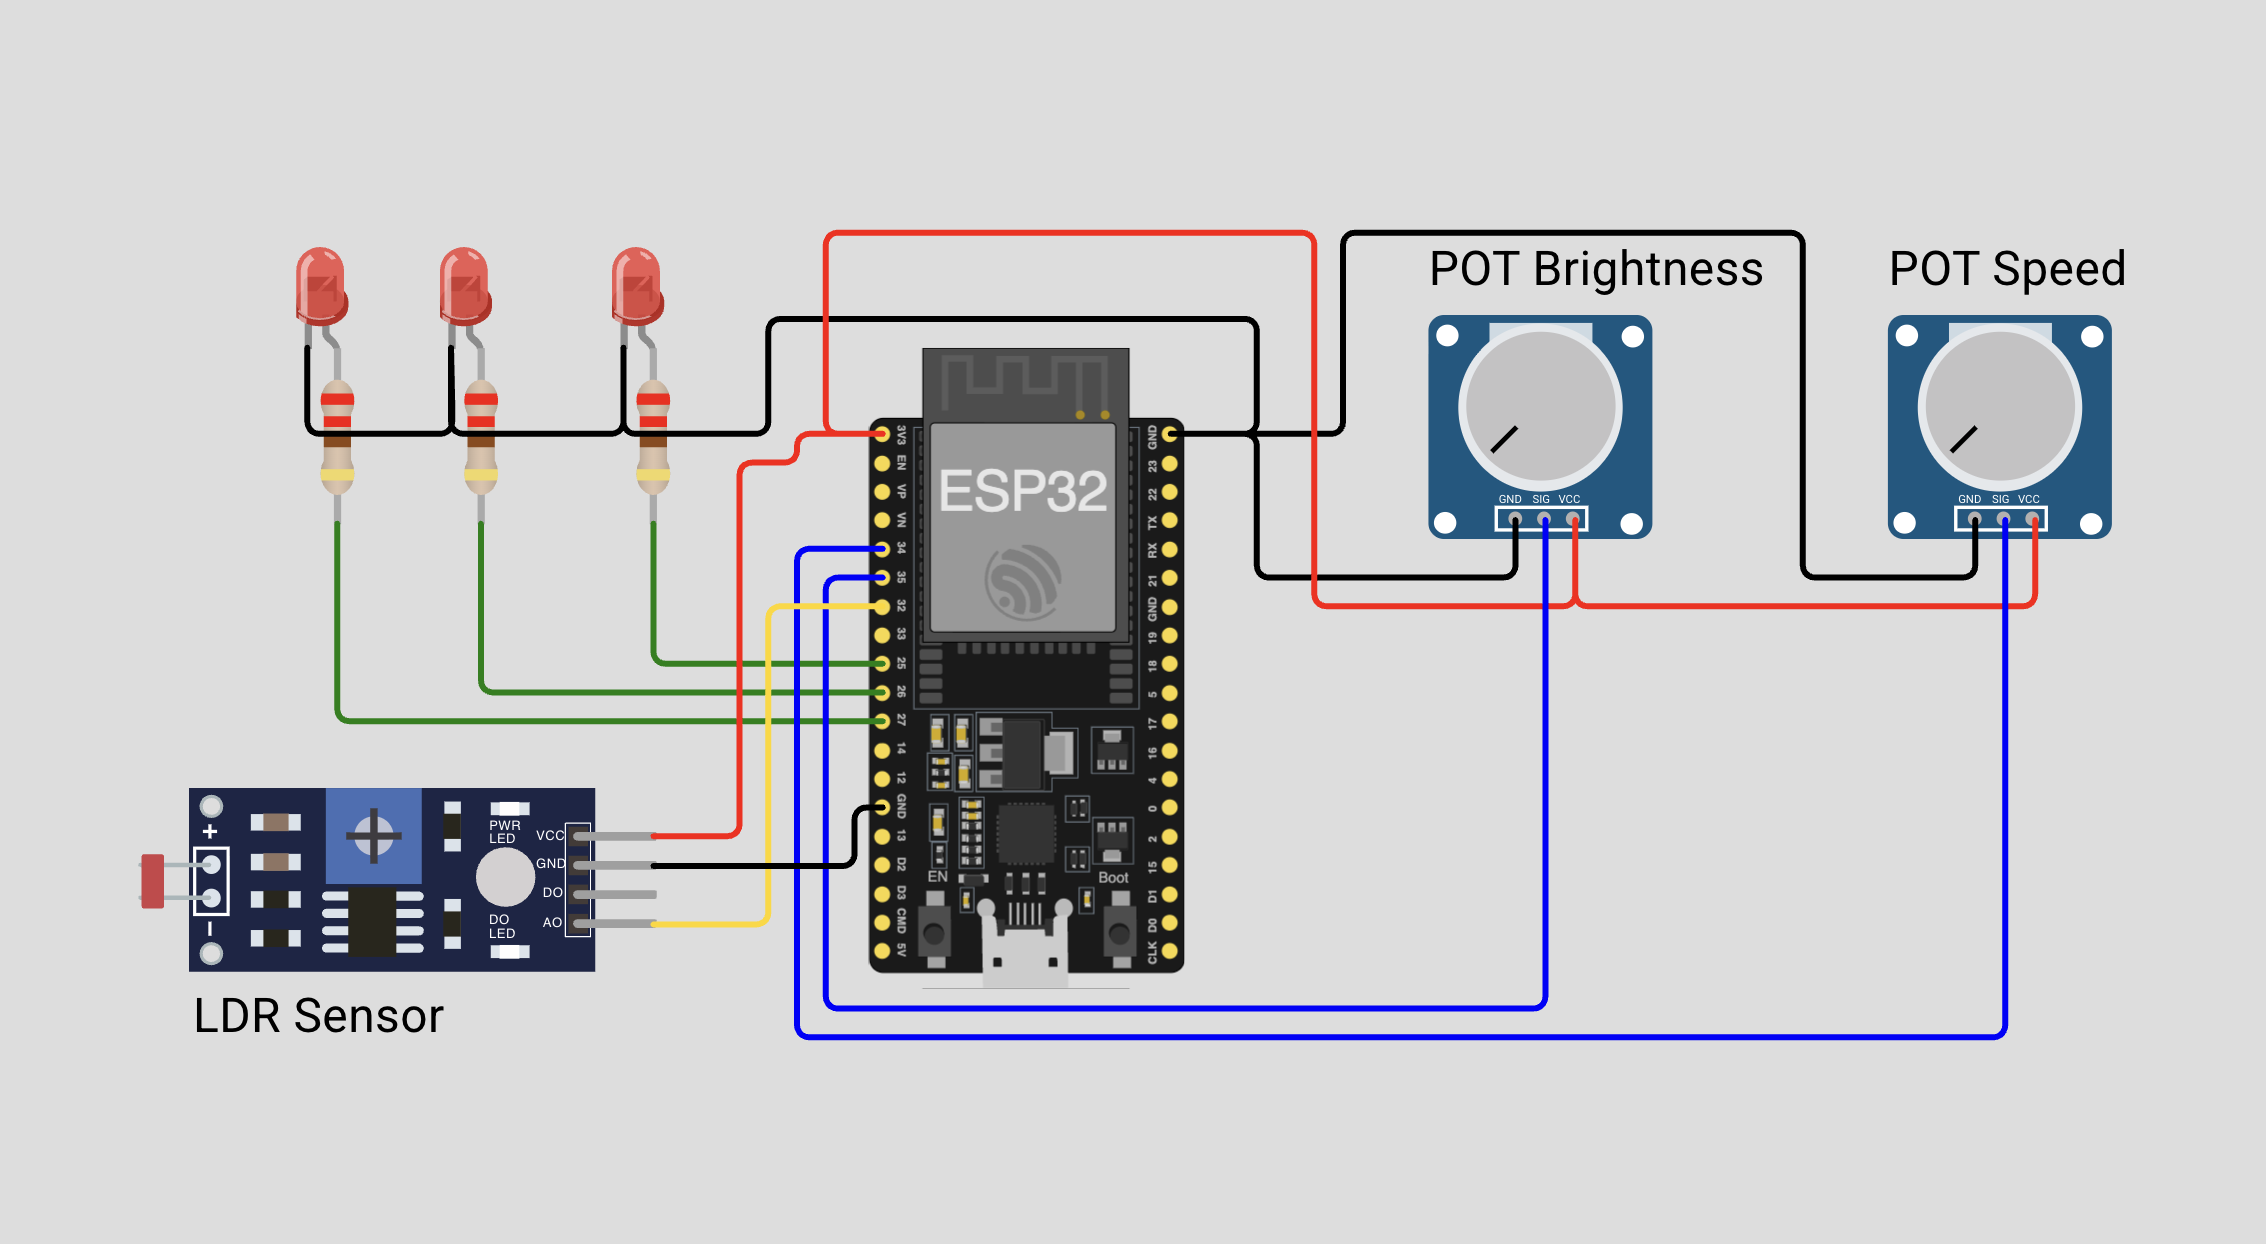
\includegraphics[width=0.82\textwidth]{assets/img/wiring-lampu-berjalan.png}
    \caption{Wiring diagram lampu berjalan dengan LDR dan potensiometer}
    \label{fig:wiring-lampu}
\end{figure}

Tabel \ref{tab:wiring-lampu} berikut menjelaskan detail koneksi pin antara ESP32 dengan komponen-komponen pada rangkaian lampu berjalan.

\begin{table}[H]
    \centering
    \caption{Detail Koneksi Pin Rangkaian Lampu Berjalan}
    \label{tab:wiring-lampu}
    \begin{tabular}{|l|l|l|}
        \hline
        \textbf{Komponen} & \textbf{Pin Komponen} & \textbf{Pin ESP32} \\
        \hline
        \multirow{2}{*}{LED 1} & Anode (+) & GPIO 25 (via R 220$\Omega$) \\
         & Cathode ($-$) & GND \\
        \hline
        \multirow{2}{*}{LED 2} & Anode (+) & GPIO 26 (via R 220$\Omega$) \\
         & Cathode ($-$) & GND \\
        \hline
        \multirow{2}{*}{LED 3} & Anode (+) & GPIO 27 (via R 220$\Omega$) \\
         & Cathode ($-$) & GND \\
        \hline
        \multirow{3}{*}{Potensiometer Kecepatan} & Kaki 1 & 3V3 \\
         & Wiper (tengah) & GPIO 34 \\
         & Kaki 3 & GND \\
        \hline
        \multirow{3}{*}{Potensiometer Kecerahan} & Kaki 1 & 3V3 \\
         & Wiper (tengah) & GPIO 35 \\
         & Kaki 3 & GND \\
        \hline
        \multirow{4}{*}{Sensor LDR} & Kaki 1 & 3V3 \\
         & Kaki 2 & GPIO 32 \\
         & Resistor 10k$\Omega$ (kaki 1) & GPIO 32 \\
         & Resistor 10k$\Omega$ (kaki 2) & GND \\
        \hline
    \end{tabular}
\end{table}

\subsection{Kode Program}
Kode program berikut digunakan untuk menjalankan efek lampu berjalan, membaca nilai LDR, membaca dua potensiometer, mengatur brightness LED menggunakan PWM, serta melakukan scanning WiFi secara asinkron.

\lstinputlisting[language=C++, caption={Kode program lampu berjalan, kontrol LDR, dimming, dan WiFi scanner}]{assets/code/knight-rider-wifi-scan.cpp}

\subsection{Hasil dan Pembahasan}
Sistem berhasil mengimplementasikan semua fitur yang direncanakan. Sensor LDR membaca nilai intensitas cahaya lingkungan melalui pin ADC ESP32. Jika nilai ADC LDR melebihi nilai threshold 2000, sistem menganggap kondisi lingkungan sedang gelap dan mengaktifkan efek lampu berjalan. Sebaliknya, jika nilai ADC berada di bawah threshold, sistem menganggap kondisi lingkungan terang dan seluruh LED dimatikan.

\begin{figure}[H]
    \centering
    \begin{minipage}{0.45\textwidth}
        \centering
        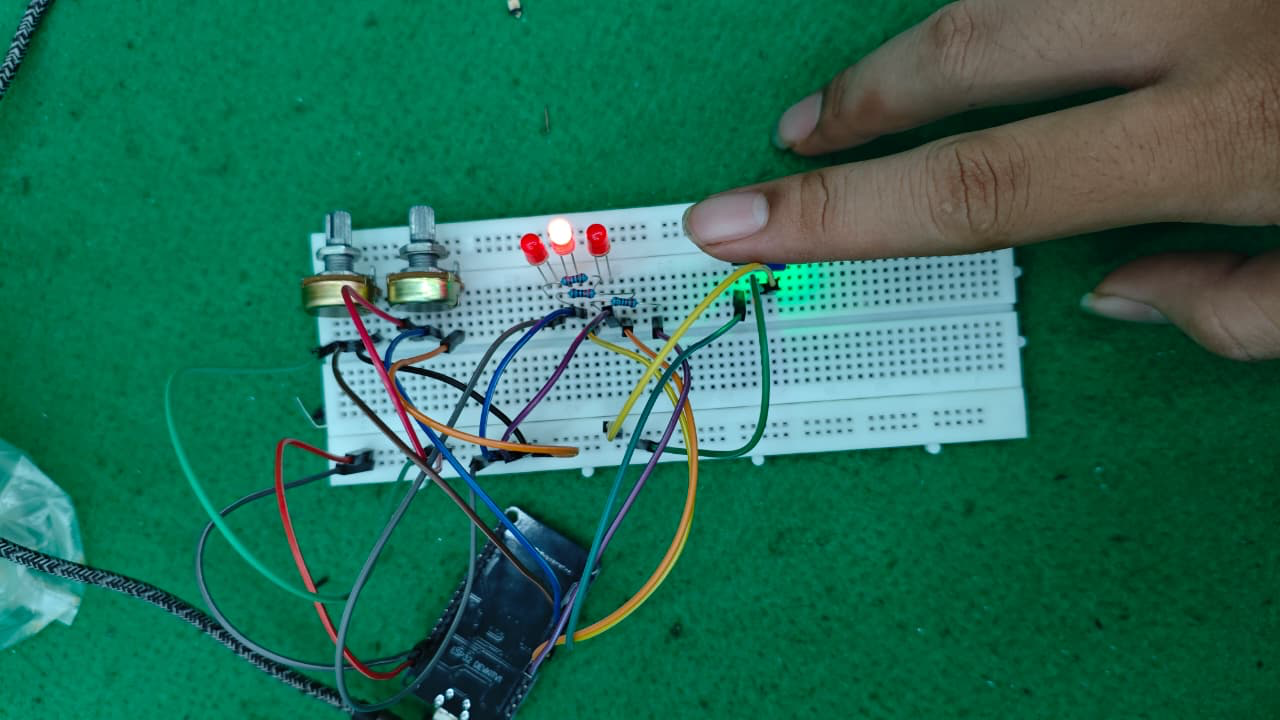
\includegraphics[width=\textwidth]{assets/img/lampu-jalan-nyala.png}
        \caption{Kondisi lampu berjalan menyala saat lingkungan gelap}
        \label{fig:lampu-nyala}
    \end{minipage}
    \hfill
    \begin{minipage}{0.45\textwidth}
        \centering
        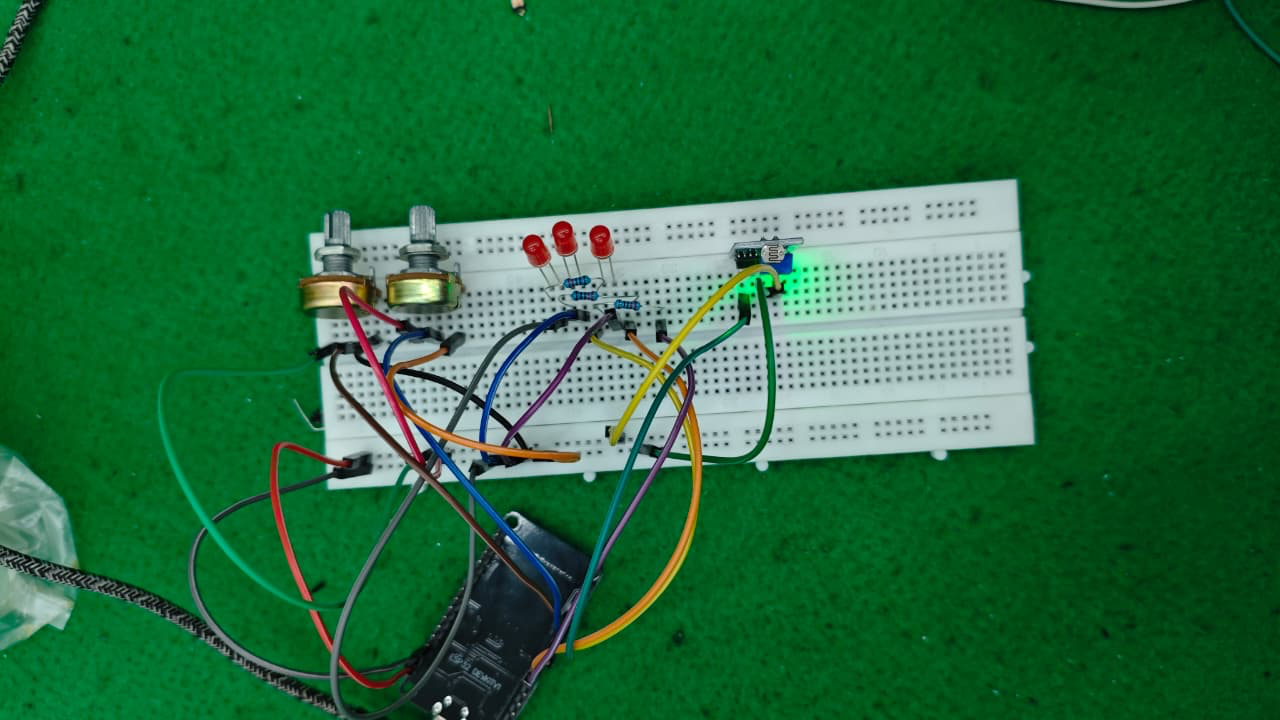
\includegraphics[width=\textwidth]{assets/img/lampu-jalan-mati.png}
        \caption{Kondisi lampu berjalan mati saat lingkungan terang}
        \label{fig:lampu-mati}
    \end{minipage}
\end{figure}

Nilai dari kedua potensiometer dibaca secara terpisah oleh ESP32. Potensiometer pertama digunakan untuk mengatur kecepatan animasi dengan memetakan nilai ADC 0 hingga 4095 ke rentang delay 50 hingga 500 ms. Jika nilai delay semakin kecil, maka perpindahan LED akan semakin cepat. Jika nilai delay semakin besar, maka perpindahan LED akan semakin lambat.

Potensiometer kedua digunakan untuk mengatur brightness LED. Nilai ADC dari potensiometer dipetakan ke rentang duty cycle PWM 0 hingga 255. Duty cycle yang lebih besar menghasilkan LED yang lebih terang, sedangkan duty cycle yang lebih kecil menghasilkan LED yang lebih redup.

\begin{figure}[H]
    \centering
    \begin{minipage}{0.45\textwidth}
        \centering
        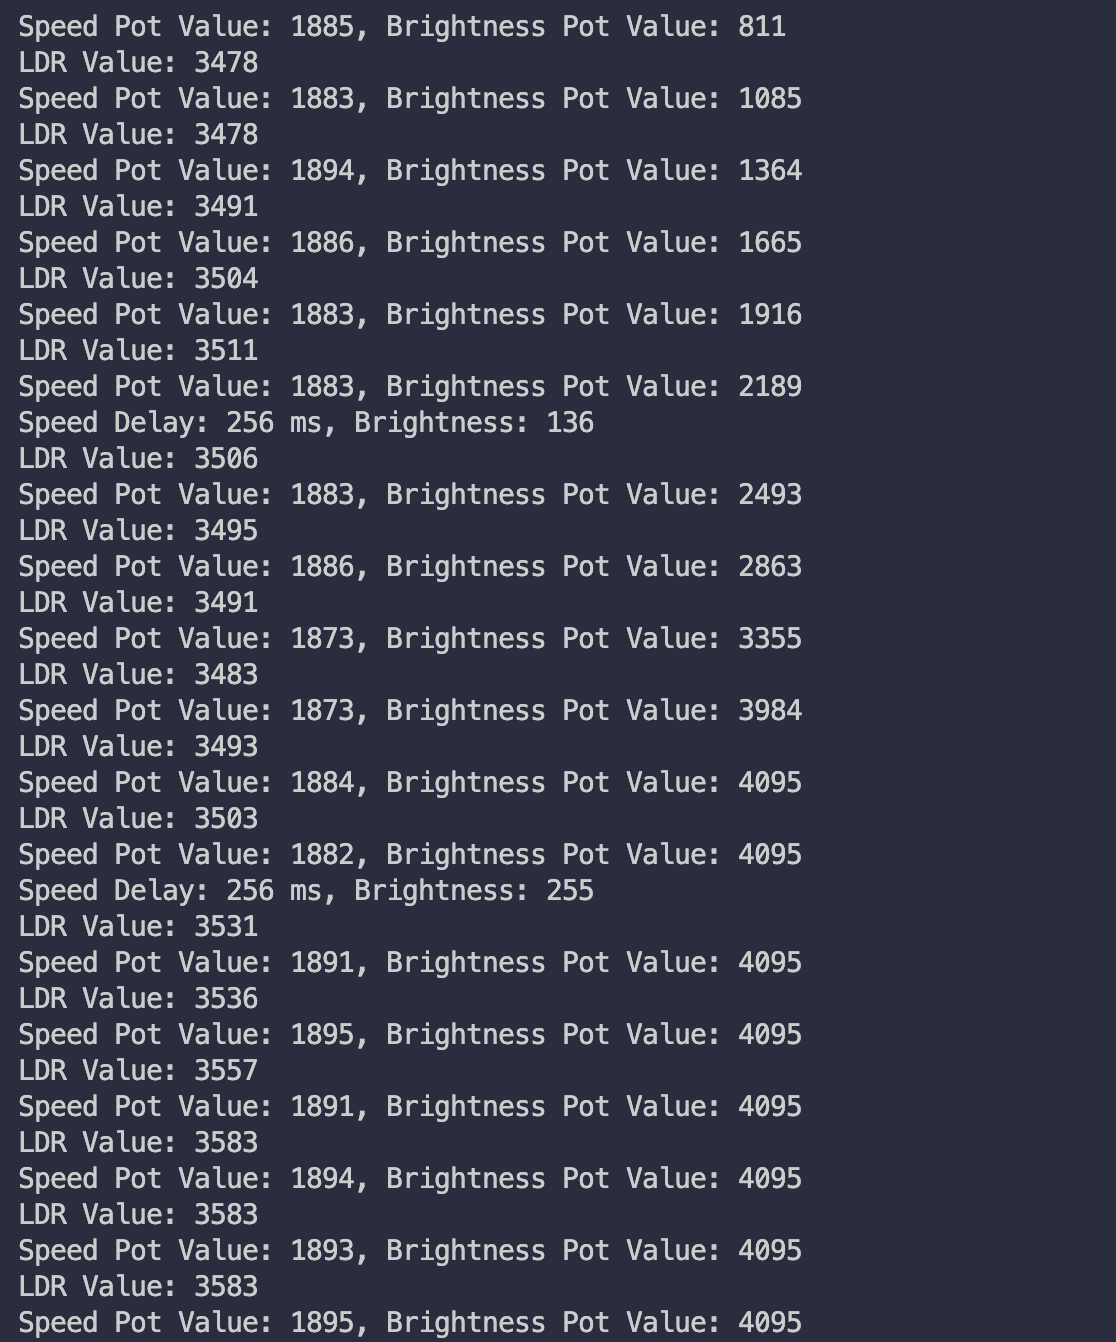
\includegraphics[width=\textwidth]{assets/img/pot-serial-monitor.png}
        \caption{Output Serial Monitor pembacaan potensiometer dan LDR}
        \label{fig:pot-serial}
    \end{minipage}
    \hfill
    \begin{minipage}{0.45\textwidth}
        \centering
        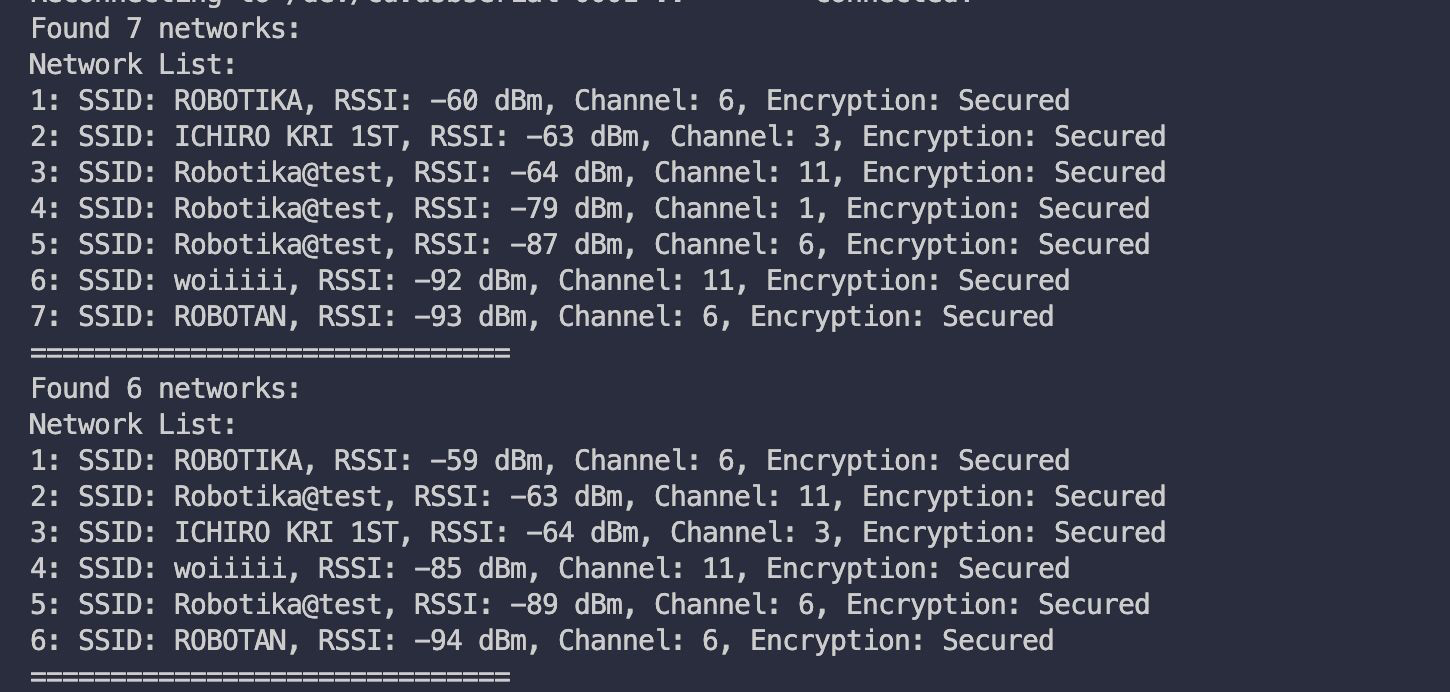
\includegraphics[width=\textwidth]{assets/img/wifi-scan.png}
        \caption{Output Serial Monitor hasil pemindaian jaringan WiFi}
        \label{fig:wifi-scan}
    \end{minipage}
\end{figure}

Pada Gambar \ref{fig:pot-serial}, Serial Monitor menampilkan nilai pembacaan dari potensiometer dan LDR. Data tersebut digunakan untuk memantau apakah input analog terbaca dengan benar oleh ESP32. Tampilan Serial Monitor juga membantu dalam proses debugging karena perubahan nilai potensiometer dapat langsung diamati.

Fitur WiFi scanner berjalan secara asinkron setiap interval tertentu. Penggunaan \texttt{WiFi.scanNetworks(true)} membuat proses pemindaian jaringan WiFi tidak memblokir eksekusi program utama. Dengan demikian, animasi lampu berjalan tetap dapat berjalan, pembacaan sensor tetap dilakukan, dan sistem tidak berhenti sementara saat proses scanning WiFi berlangsung.

Hasil pemindaian WiFi ditampilkan pada Serial Monitor, meliputi nama jaringan atau SSID, kekuatan sinyal atau RSSI, channel, dan status enkripsi. Hal ini menunjukkan bahwa ESP32 tidak hanya dapat digunakan untuk membaca sensor dan mengontrol output, tetapi juga dapat memanfaatkan konektivitas nirkabel untuk kebutuhan monitoring atau komunikasi data.

\section{Kesimpulan}
Berdasarkan mini project yang telah dibuat, dapat disimpulkan bahwa:
\begin{enumerate}
    \item PWM pada ESP32 dapat digunakan untuk mengatur kecerahan LED secara dinamis berdasarkan input analog dari potensiometer.
    \item ADC pada ESP32 mampu membaca beberapa input analog sekaligus, yaitu potensiometer kecepatan, potensiometer brightness, dan sensor LDR.
    \item Sensor LDR dapat digunakan sebagai input otomatis untuk mengaktifkan atau menonaktifkan sistem berdasarkan kondisi cahaya lingkungan.
    \item Potensiometer dapat digunakan sebagai kontrol manual yang sederhana untuk mengatur parameter sistem seperti kecepatan animasi dan tingkat kecerahan LED.
    \item Fitur WiFi scanning asinkron pada ESP32 memungkinkan proses pemindaian jaringan berjalan tanpa mengganggu tugas utama sistem.
    \item Mini project ini berhasil menggabungkan konsep PWM, ADC, sensor, aktuator, dan konektivitas WiFi dalam satu sistem embedded sederhana.
\end{enumerate}

\end{document}